\documentclass{article}
\usepackage{amsmath}
\usepackage{amsfonts}
\usepackage{multicol}
\usepackage{graphicx}
\usepackage{subcaption}
\graphicspath{ {../images/} }

\usepackage[utf8]{inputenc}
\usepackage{graphicx}
\usepackage{setspace}
\usepackage{amsmath}
\usepackage{indentfirst}

\begin{document}

\begin{titlepage}
    \centering
    \vspace*{2cm}
    
    \Huge
    \textbf{Elementos Finitos}
    
    \vspace{1.5cm}
    
    \Large
    \textbf{Breno Bertone}
    
    \vspace{0.5cm}
    
    \Large
    RA: 250842
    
    \vfill
    
    \vspace{0.8cm}
    
    
    \vspace{1.5cm}    
    
\end{titlepage}

Todos os códigos de suporte desse trabalho podem ser encontrados em 

\section{Exercício 1}
\subsection{Parte (a)}

Dado \( u_h(x) = \sum_{i=1}^n w_i \phi_i(x) \), substituímos na forma fraca:
\[
\int_0^1 [u_h' v_h' + u_h v_h] \, dx = \int_0^1 x v_h \, dx \quad \forall v_h \in \mathcal{V}_h.
\]

Escolhendo \( v_h = \phi_j \) para \( j = 1, 2, \ldots, n \):
\[
\int_0^1 \left[ \left( \sum_{i=1}^n w_i \phi_i' \right) \phi_j' + \left( \sum_{i=1}^n w_i \phi_i \right) \phi_j \right] dx = \int_0^1 x \phi_j \, dx.
\]

Separando as somas e integrando termo a termo:
\[
\sum_{i=1}^n w_i \left( \int_0^1 \phi_i' \phi_j' \, dx + \int_0^1 \phi_i \phi_j \, dx \right) = \int_0^1 x \phi_j \, dx.
\]

Definimos os elementos da matriz \( A \) e do vetor \( \mathbf{f} \) como:
\[
a_{ij} = \int_0^1 \left( \phi_i' \phi_j' + \phi_i \phi_j \right) dx,
\]
\[
f_j = \int_0^1 x \phi_j \, dx.
\]

Assim, podemos escrever o sistema linear na forma matricial:
\[
A \mathbf{w} = \mathbf{f},
\]
onde \( A \in \mathbb{R}^{n \times n} \) tem elementos \( a_{ij} \) e \( \mathbf{f} \in \mathbb{R}^n \) tem elementos \( f_j \).

\subsection{Parte (B)}
Para encontrar a solução aproximada do Problema V usando o Método de Galerkin, precisamos montar as matrizes \( A \) e os vetores \( \mathbf{f} \) para cada valor de \( n \).

\textbf{Para \( n = 1 \):}

Usamos \( \phi_1(x) = x (x - 1) \).

A matriz \( A \) e o vetor \( \mathbf{f} \) são dados por:
\[
A_{1 \times 1} = \begin{bmatrix}
a_{11}
\end{bmatrix},
\]
\[
\mathbf{f}_{1} = \begin{bmatrix}
f_1
\end{bmatrix},
\]


\textbf{Para \( n = 2 \):}

Usamos \( \phi_1(x) = x (x - 1) \) e \( \phi_2(x) = x^2 (x - 1) \).

A matriz \( A \) e o vetor \( \mathbf{f} \) são dados por:
\[
A_{2 \times 2} = \begin{bmatrix}
a_{11} & a_{12} \\
a_{21} & a_{22}
\end{bmatrix},
\]
\[
\mathbf{f}_{2} = \begin{bmatrix}
f_1 \\
f_2
\end{bmatrix},
\]


\textbf{Para \( n = 3 \):}

Usamos \( \phi_1(x) = x (x - 1) \), \( \phi_2(x) = x^2 (x - 1) \) e \( \phi_3(x) = x^3 (x - 1) \).

A matriz \( A \) e o vetor \( \mathbf{f} \) são dados por:
\[
A_{3 \times 3} = \begin{bmatrix}
a_{11} & a_{12} & a_{13} \\
a_{21} & a_{22} & a_{23} \\
a_{31} & a_{32} & a_{33}
\end{bmatrix},
\]
\[
\mathbf{f}_{3} = \begin{bmatrix}
f_1 \\
f_2 \\
f_3
\end{bmatrix},
\]

Para evitar repetição, vamos mostar só os termos de n=3:
\[
A_{3 \times 3} = \begin{bmatrix}
    \frac{11}{30} & \frac{11}{60} & \frac{23}{210} \\
    \frac{11}{60} & \frac{1}{7} & \frac{89}{840} \\
    \frac{23}{210} & \frac{89}{840} & \frac{113}{1260}
    \end{bmatrix}
\]

\[
\mathbf{f}_{3} = \begin{bmatrix}
    -\frac{1}{12} \\
    -\frac{1}{20} \\
    -\frac{1}{30}
    \end{bmatrix}
\]

\section{Exercício 2}

Na mesma lógica do exercício anterior, vamos omitir as contas para n=1 e n=2

\textbf{Para \( n = 3 \):}

Usamos \( \phi_1(x) = \sin(\pi x) \), \( \phi_2(x) = \sin(2\pi x) \) e \( \phi_3(x) = \sin(3\pi x) \).

A matriz \( A \) e o vetor \( \mathbf{f} \) são dados por:
\[
A_{3 \times 3} = \begin{bmatrix}
a_{11} & a_{12} & a_{13} \\
a_{21} & a_{22} & a_{23} \\
a_{31} & a_{32} & a_{33}
\end{bmatrix},
\]
\[
\mathbf{f}_{3 \times 1} = \begin{bmatrix}
f_1 \\
f_2 \\
f_3
\end{bmatrix},
\]
onde:
\begin{multicols}{2}
    \noindent
    \[
    a_{11} = \frac{\pi^2}{2} + \frac{1}{2},
    \]
    \[
    a_{12} = 0,
    \]
    \[
    a_{13} = 0,
    \]
    \[
    a_{21} = a_{12} = 0,
    \]
    \[
    a_{22} = 2\pi^2 + \frac{1}{2},
    \]
    \[
    a_{23} = 0,
    \]
    \[
    a_{31} = a_{13} = 0,
    \]
    \[
    a_{32} = a_{23} = 0,
    \]
    \[
    a_{33} = 4.5\pi^2 + \frac{1}{2},
    \]
    
    \columnbreak
    
    \noindent
    \[
    f_1 = \int_0^1 x \sin(\pi x) \, dx,
    \]
    \[
    f_2 = \int_0^1 x \sin(2\pi x) \, dx,
    \]
    \[
    f_3 = \int_0^1 x \sin(3\pi x) \, dx.
    \]
    \end{multicols}

Assim, teremos:

\[
A_{3 \times 3} = \begin{bmatrix}
    \frac{1}{2} + \frac{\pi^2}{2} & 0 & 0 \\
    0 & \frac{1}{2} + 2\pi^2 & 0 \\
    0 & 0 & \frac{1}{2} + \frac{9\pi^2}{2}
    \end{bmatrix}
\]

\[
\mathbf{f}_{3} = \begin{bmatrix}
    \frac{1}{\pi} \\
    -\frac{1}{2\pi} \\
    \frac{1}{3\pi}
    \end{bmatrix}
\]

\section{Exercício 3}
Resolvendo os sistemas lineares definidos nos exercícios anteriores obtemos os seguintes gráficos:

\begin{center}
    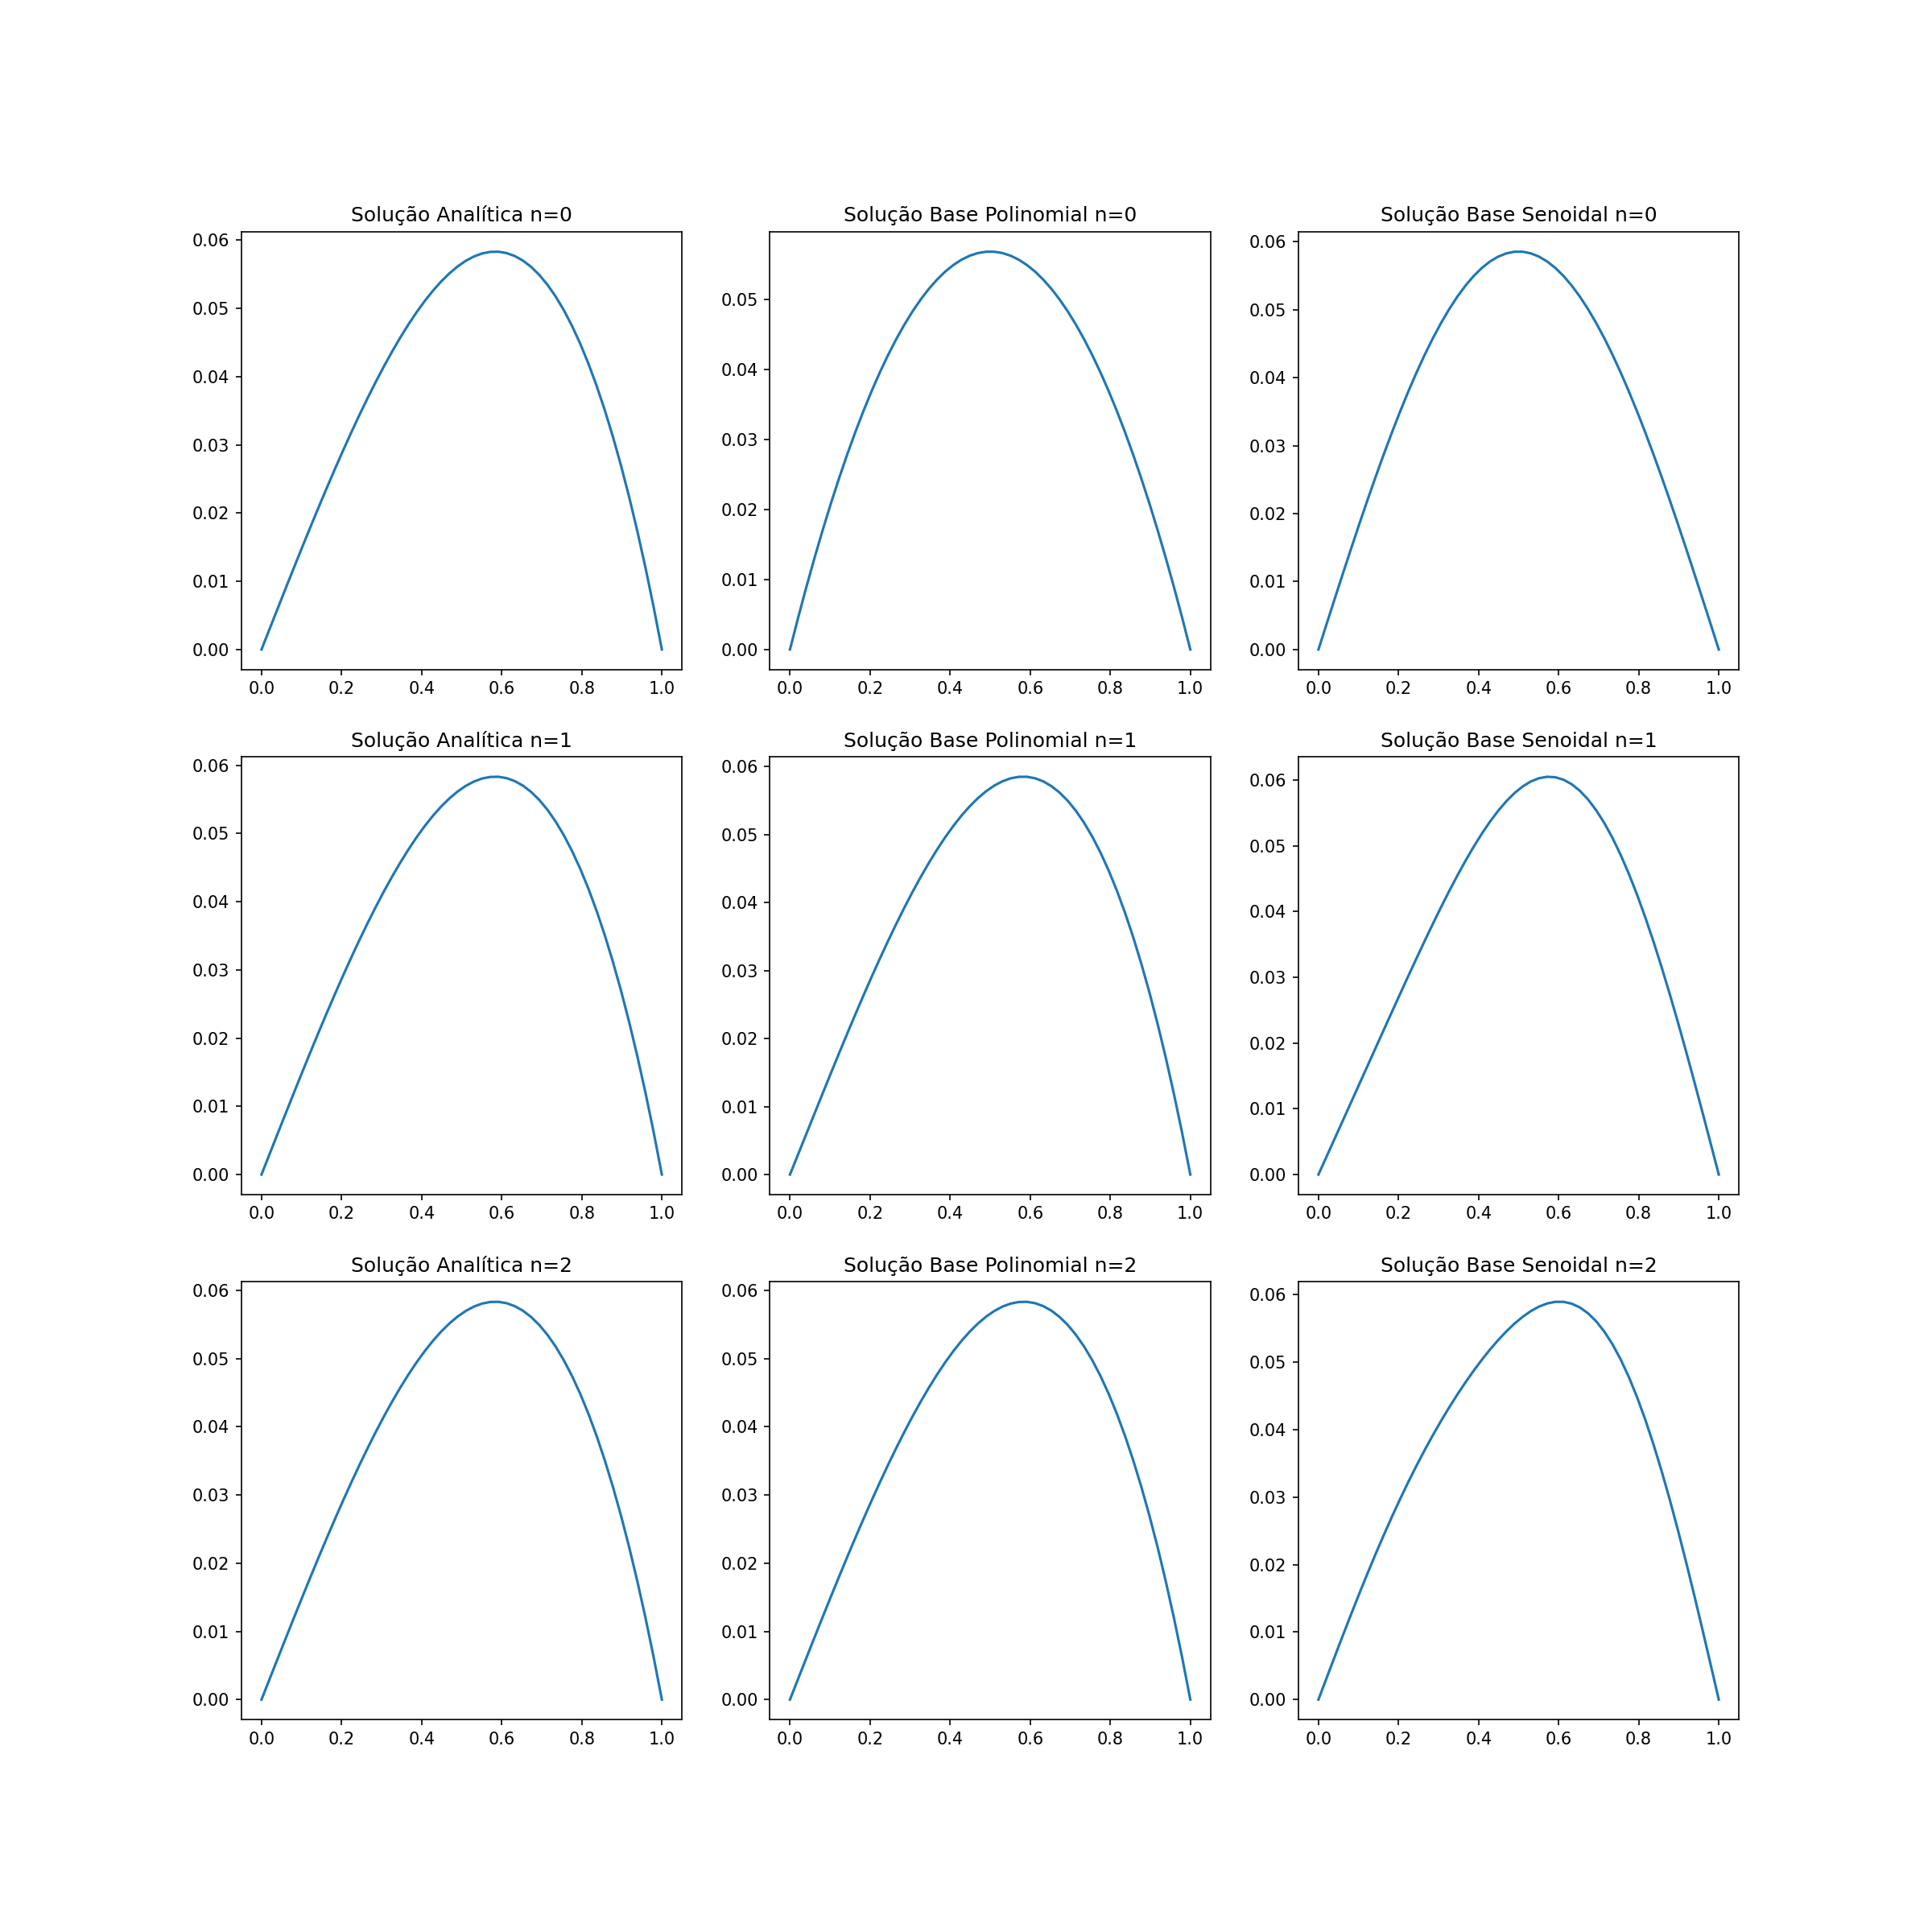
\includegraphics[width=1\textwidth]{exercicio123_solucao.png}
\end{center}

E as derivadas:
\begin{center}
    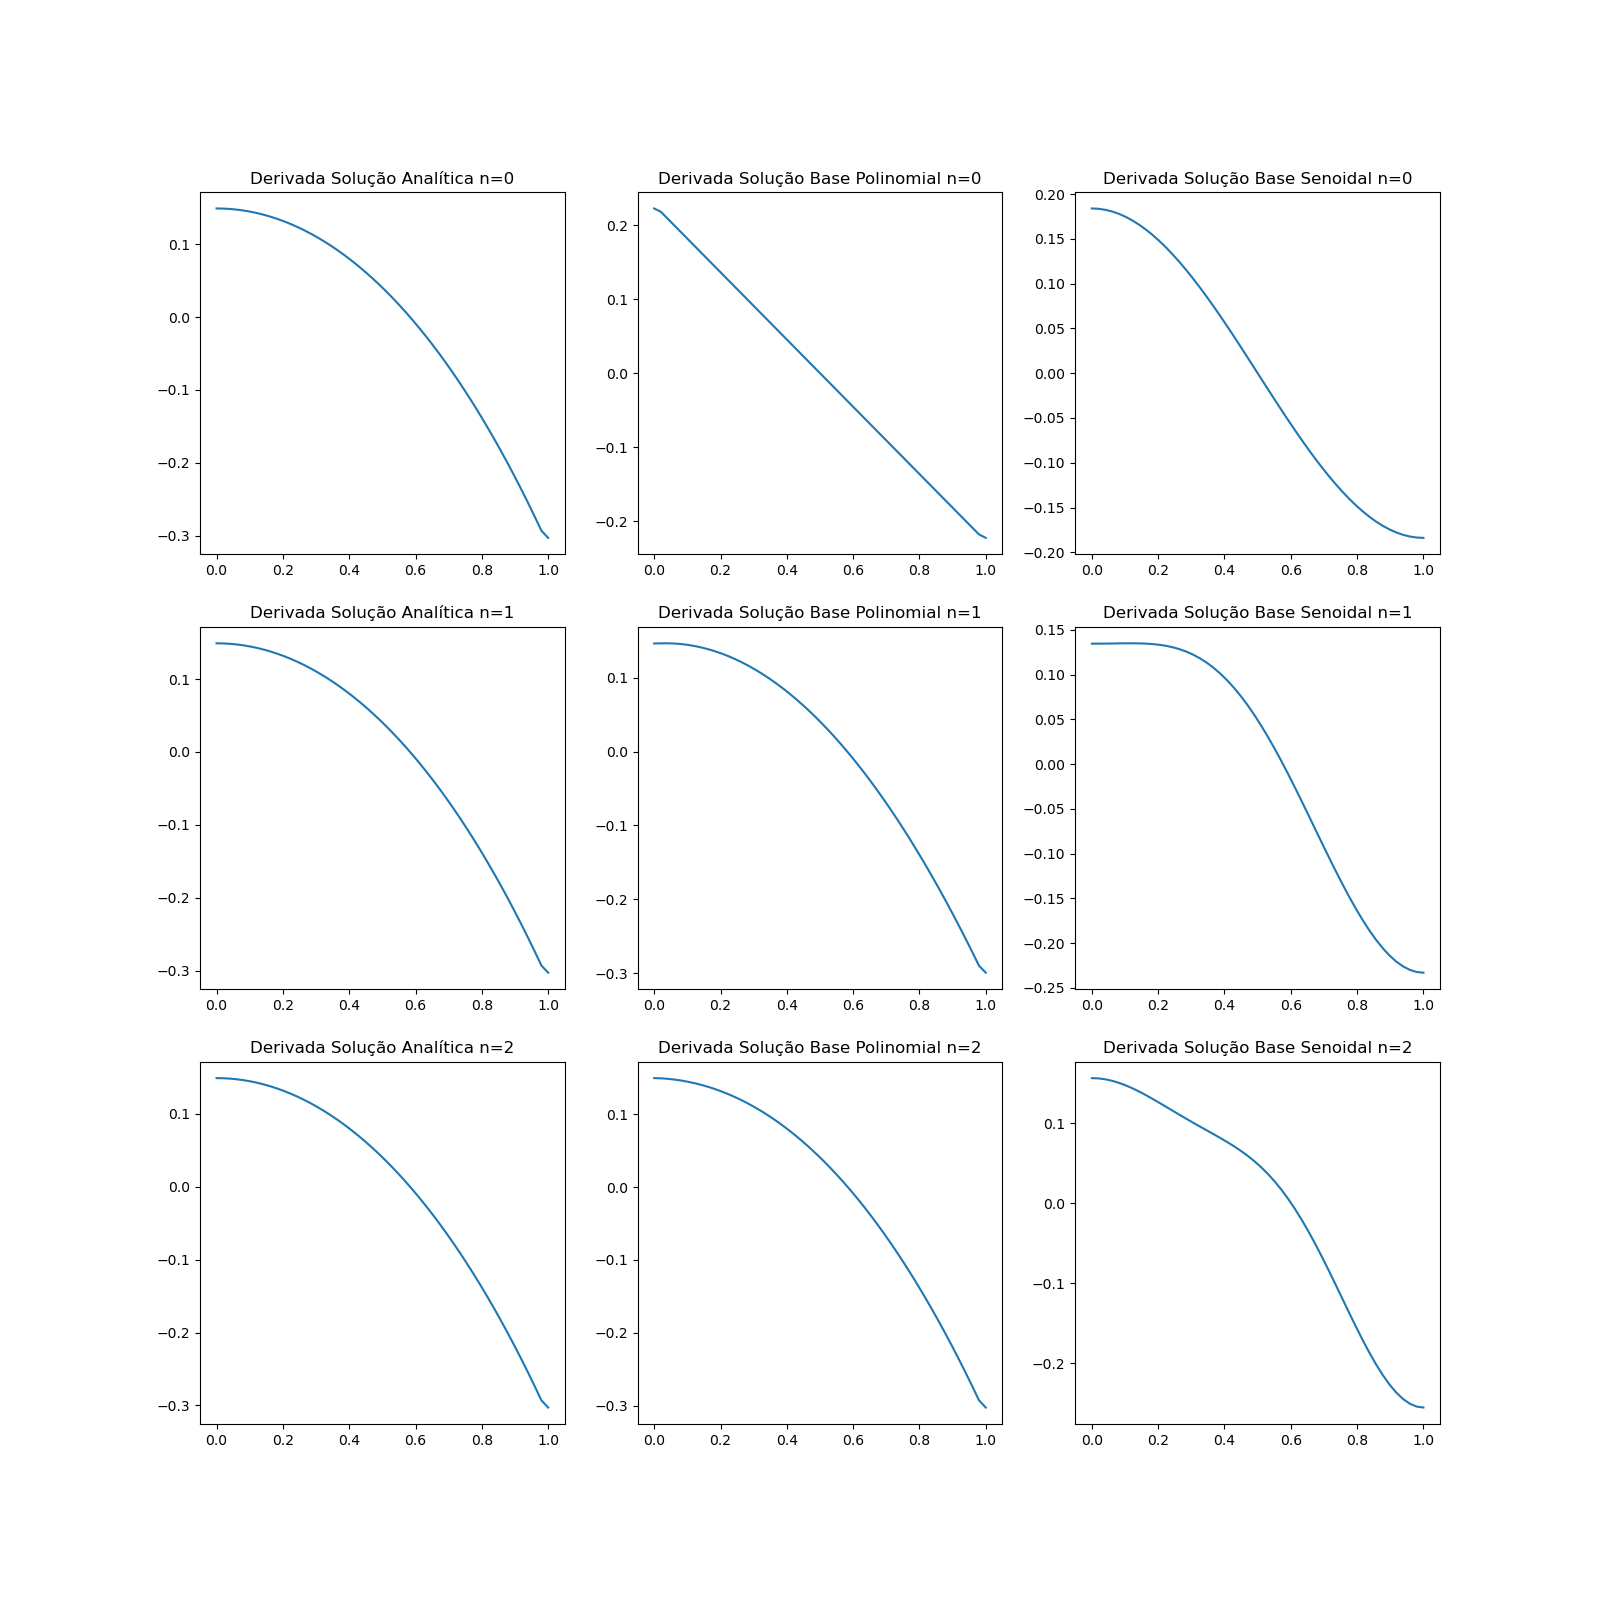
\includegraphics[width=1\textwidth]{exercicio123_derivadas_solucao.png}
\end{center}


\section{Exercício 4}


\subsection{Parte (a)}

\subsubsection{Cálculo de \( a_{ij} \)}

Para \( \phi_i(x) = x^i(x-1) \) e \( \phi_j(x) = x^j(x-1) \), temos:

\[
\phi_i(x) = x^i (x-1), \quad \phi_i'(x) = ix^{i-1}(x-1) + x^i,
\]

\[
\phi_j(x) = x^j (x-1), \quad \phi_j'(x) = jx^{j-1}(x-1) + x^j.
\]

O coeficiente \( a_{ij} \) é dado por:

\[
a_{ij} = \int_0^1 (\phi_i' \phi_j' + \phi_i \phi_j) \, dx.
\]

Expandindo \( \phi_i'(x) \phi_j'(x) \):

\[
\phi_i'(x) \phi_j'(x) = [ix^{i-1}(x-1) + x^i][jx^{j-1}(x-1) + x^j],
\]

\[
\phi_i'(x) \phi_j'(x) = ijx^{i+j-2}(x-1)^2 + i x^{i+j-1}(x-1) + j x^{i+j-1}(x-1) + x^{i+j}.
\]

Calculamos a integral do primeiro termo:

\[
\int_0^1 ij x^{i+j-2} (x-1)^2 \, dx = ij \left( \frac{1}{i+j+1} - \frac{2}{i+j} + \frac{1}{i+j-1} \right),
\]

e dos termos cruzados e constante:

\[
(i+j) \left( \frac{1}{i+j+1} - \frac{1}{i+j} \right) + \frac{1}{i+j+1},
\]

e da integral sem derivadas:

\[
\frac{1}{i+j+3} - 2 \frac{1}{i+j+2} + \frac{1}{i+j+1}.
\]

Somando todos os termos, obtemos:

\[
a_{ij} = \frac{ij}{i+j-1} - \frac{[(1+i)j + (1+j)i]}{i+j} + \frac{1 + (1+i)(1+j)}{i+j+1} - \frac{2}{i+j+2} + \frac{1}{i+j+3}.
\]

\subsubsection{Cálculo de \( f_i \)}
Para \( f_i \), temos:
\[
f_i = \int_0^1 x \phi_i(x) \, dx = \int_0^1 x^{i+1}(x-1) \, dx = \frac{1}{i+3} - \frac{1}{i+2}.
\]

Calculando esse problema, obtemos os seguintes gráficos:

\begin{center}
    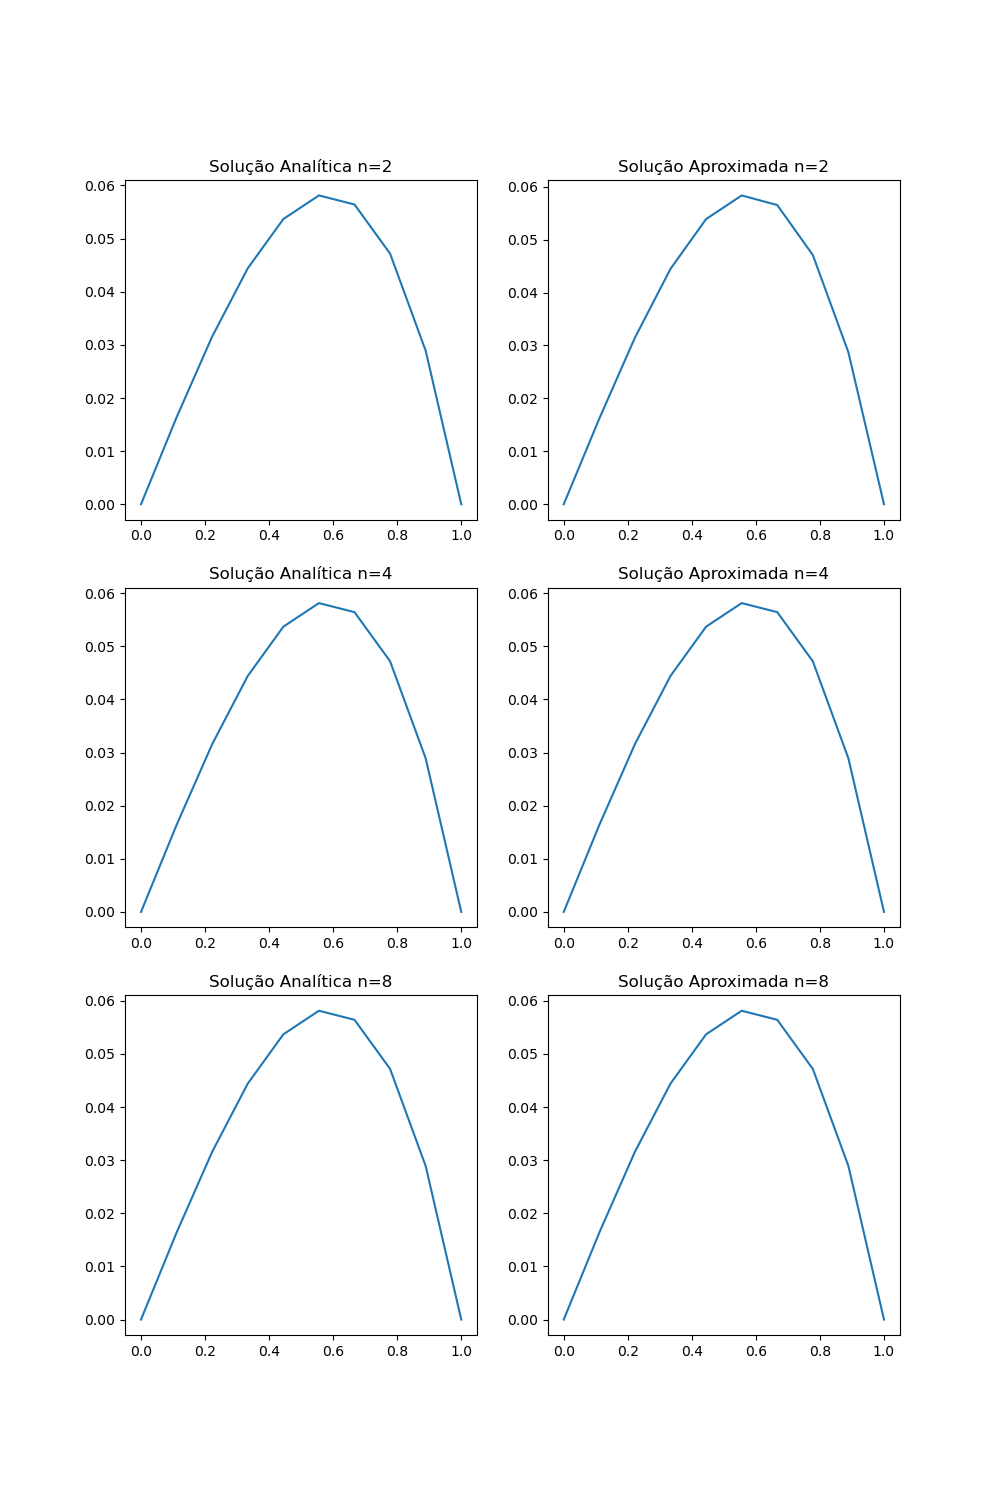
\includegraphics[width=1\textwidth]{exercicio4.png}
\end{center}

\section{Exercício 5}
\subsection{Parte (a)}

Seja \( \phi_i(x) = \sin(i \pi x) \).

Os coeficientes \( a_{ij} \) da matriz \( A \) são dados por:
\[
a_{ij} = \int_0^1 \left( \phi_i' \phi_j' + \phi_i \phi_j \right) dx.
\]

Como \( \phi_i(x) = \sin(i \pi x) \), temos \( \phi_i'(x) = i \pi \cos(i \pi x) \). Então:
\[
a_{ij} = \int_0^1 \left( (i \pi \cos(i \pi x))(j \pi \cos(j \pi x)) + \sin(i \pi x) \sin(j \pi x) \right) dx.
\]

Utilizando as propriedades:
\[
\int_0^1 \cos(n\pi x) \cos(m\pi x) \, dx = \begin{cases}
0, & \text{se } n \neq m, \\
\frac{1}{2}, & \text{se } n = m,
\end{cases}
\]
\[
\int_0^1 \sin(n\pi x) \sin(m\pi x) \, dx = \begin{cases}
0, & \text{se } n \neq m, \\
\frac{1}{2}, & \text{se } n = m,
\end{cases}
\]

Para \( i = j \), temos:
\[
a_{ii} = \int_0^1 \left( (i \pi \cos(i \pi x))^2 + \sin^2(i \pi x) \right) dx = i^2 \pi^2 \cdot \frac{1}{2} + \frac{1}{2} = \frac{i^2 \pi^2}{2} + \frac{1}{2}.
\]

Para \( i \neq j \), temos:
\[
a_{ij} = 0.
\]

Portanto, a matriz \( A \) é diagonal com elementos:
\[
a_{ii} = \frac{i^2 \pi^2}{2} + \frac{1}{2}.
\]

O vetor \( \mathbf{f} \) é dado por:
\[
f_i = \int_0^1 x \sin(i \pi x) \, dx.
\]

Para encontrar a expressão analítica de \( f_i \), integramos por partes:
\[
f_i = \left[ -\frac{x \cos(i \pi x)}{i \pi} \right]_0^1 + \int_0^1 \frac{\cos(i \pi x)}{i \pi} \, dx = 0 + \left[ \frac{\sin(i \pi x)}{(i \pi)^2} \right]_0^1 = \frac{1}{(i \pi)^2}.
\]

Portanto, temos:
\[
f_i = \frac{1}{i^2 \pi^2}.
\]

Para encontrar \( w_i \), resolvemos o sistema linear \( A \mathbf{w} = \mathbf{f} \):
\[
\left( \frac{i^2 \pi^2}{2} + \frac{1}{2} \right) w_i = \frac{1}{i^2 \pi^2},
\]
\[
w_i = \frac{\frac{1}{i^2 \pi^2}}{\frac{i^2 \pi^2}{2} + \frac{1}{2}} = \frac{2}{i^4 \pi^4 + i^2 \pi^2}.
\]

Simplificando:
\[
w_i = \frac{2}{i^2 \pi^2 (i^2 \pi^2 + 1)} = \frac{2}{i^2 \pi^2 (i^2 \pi^2 + 1)}.
\]

A solução \( u_h(x) \) pode ser escrita como:
\[
u_h(x) = \sum_{i=1}^n w_i \sin(i \pi x).
\]

Substituindo \( w_i \):
\[
u_h(x) = \sum_{i=1}^n \frac{2}{i^2 \pi^2 (i^2 \pi^2 + 1)} \sin(i \pi x).
\]

\subsection{Parte (b)}

Agora, vamos mostrar que \( |w_i| > |w_{i+1}| \) e que \( \lim_{i \to \infty} w_i = 0 \).

Primeiro, comparamos \( |w_i| \) e \( |w_{i+1}| \):
\[
w_i = \frac{2}{i^2 \pi^2 (i^2 \pi^2 + 1)},
\]
\[
w_{i+1} = \frac{2}{(i+1)^2 \pi^2 ((i+1)^2 \pi^2 + 1)}.
\]

Queremos mostrar que:
\[
\left| \frac{2}{i^2 \pi^2 (i^2 \pi^2 + 1)} \right| > \left| \frac{2}{(i+1)^2 \pi^2 ((i+1)^2 \pi^2 + 1)} \right|.
\]

Como \( \frac{2}{\pi^2} \) é um fator constante, podemos simplificar a desigualdade para:
\[
\frac{1}{i^2 (i^2 \pi^2 + 1)} > \frac{1}{(i+1)^2 ((i+1)^2 \pi^2 + 1)}.
\]

Observe que:
\[
i^2 < (i+1)^2 \quad \text{e} \quad i^2 \pi^2 + 1 < (i+1)^2 \pi^2 + 1.
\]

Portanto, temos:
\[
i^2 (i^2 \pi^2 + 1) < (i+1)^2 ((i+1)^2 \pi^2 + 1).
\]

Tomando o recíproco de ambos os lados (preservando a desigualdade, já que ambos os lados são positivos):
\[
\frac{1}{i^2 (i^2 \pi^2 + 1)} > \frac{1}{(i+1)^2 ((i+1)^2 \pi^2 + 1)},
\]

logo:
\[
|w_i| > |w_{i+1}|.
\]

Agora, mostramos que \( \lim_{i \to \infty} w_i = 0 \).

Quando \( i \) tende ao infinito, o termo dominante no denominador de \( w_i \) é \( i^4 \pi^4 \):
\[
w_i = \frac{2}{i^2 \pi^2 (i^2 \pi^2 + 1)} \approx \frac{2}{i^4 \pi^4} \quad \text{para } i \text{ grande}.
\]

Portanto:
\[
w_i \approx \frac{2}{i^4 \pi^4}.
\]

Como \( i^4 \) tende ao infinito quando \( i \to \infty \), temos:
\[
\lim_{i \to \infty} \frac{2}{i^4 \pi^4} = 0.
\]

Assim, mostramos que:
\[
\lim_{i \to \infty} w_i = 0.
\]

\subsection{Parte (c)}

Utilizando a expressão de \( u_h \) conseguimos calcular diretamente cada um dos casos e obtemos os seguintes gráficos:

\begin{center}
    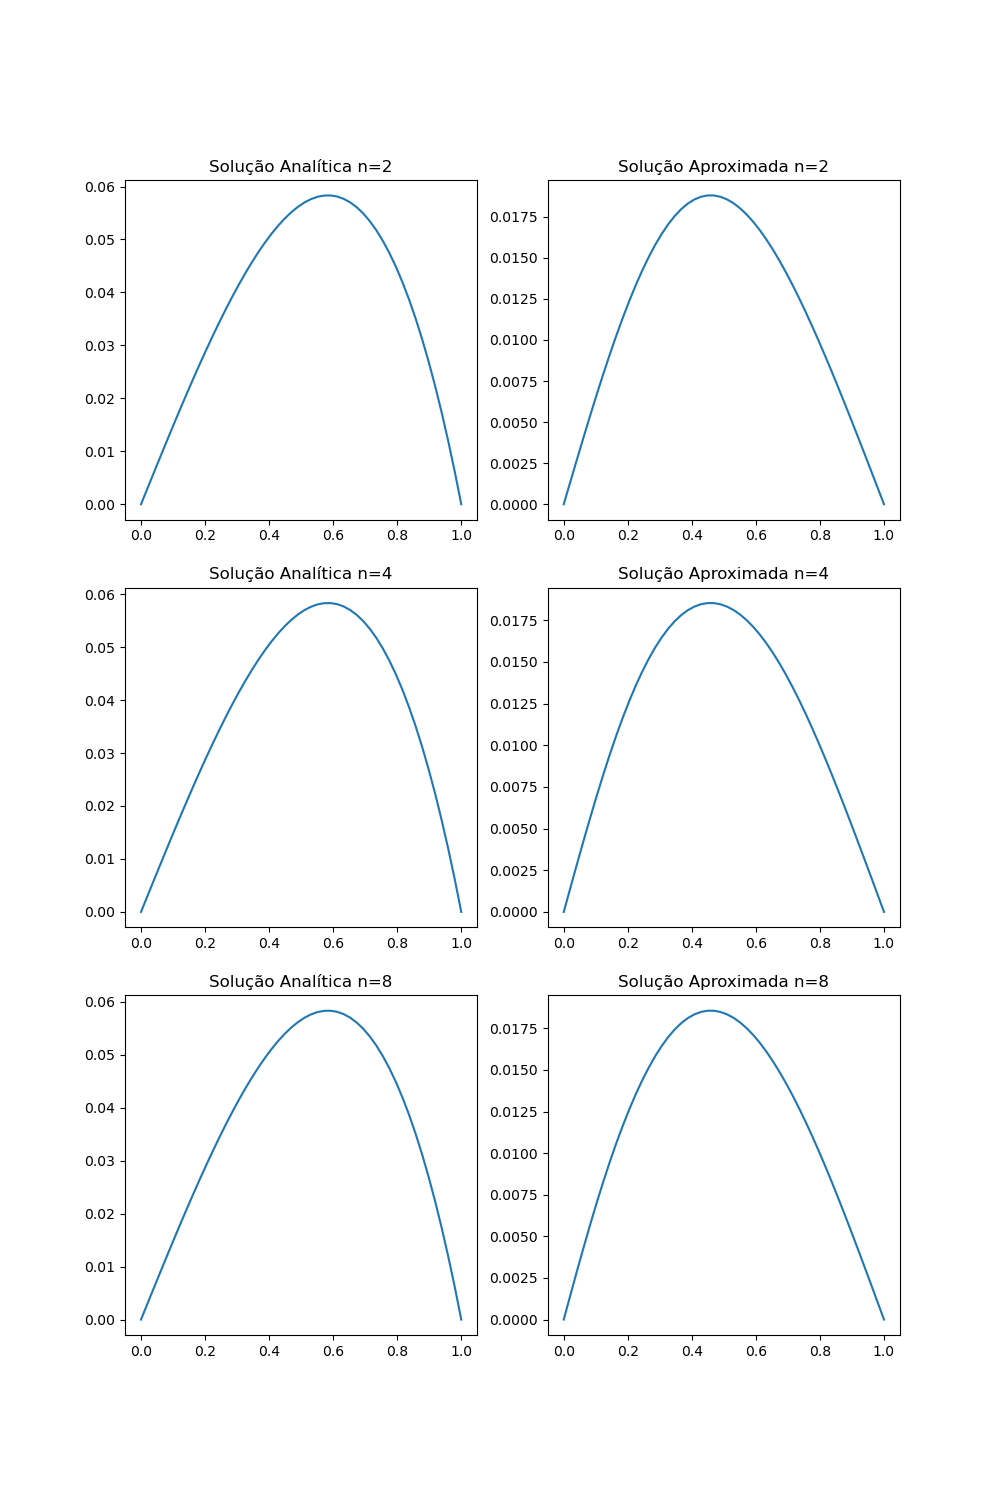
\includegraphics[width=1\textwidth]{exercicio5.png}
\end{center}

\section{Exercício 6}
\subsection{Parte (a)}

\begin{figure}[h!]
    \centering
    \begin{subfigure}[b]{\textwidth}
        \centering
        \[
            \begin{bmatrix}
                1.9e-02 & 0 & 0 & 0 & 0 & 0 \\
                0 & 1.3e-03 & 0 & 0 & 0 & 0 \\
                0 & 0 & 2.5e-04 & 0 & 0 & 0 \\
                0 & 0 & 0 & 8.0e-05 & 0 & 0 \\
                0 & 0 & 0 & 0 & 3.3e-05 & 0 \\
                0 & 0 & 0 & 0 & 0 & 1.6e-05
                \end{bmatrix}
        \]
        \caption{Matriz esperada}
    \end{subfigure}
    \vfill
    \begin{subfigure}[b]{\textwidth}
        \centering
        \[
            \begin{bmatrix}
                5.4e+00 & 1.4e-16 & -7.8e-16 & 9.9e-16 & -2.1e-16 & 8.5e-16 \\
                1.4e-16 & 2.0e+01 & 1.8e-15 & 1.7e-15 & 1.8e-15 & 4.3e-16 \\
                -7.8e-16 & 1.8e-15 & 4.5e+01 & -3.6e-15 & -2.8e-16 & -5.7e-15 \\
                9.9e-16 & 1.7e-15 & -3.6e-15 & 7.9e+01 & 2.8e-16 & 1.7e-15 \\
                -2.1e-16 & 1.8e-15 & -2.8e-16 & 2.8e-16 & 1.2e+02 & 8.5e-15 \\
                8.5e-16 & 4.3e-16 & -5.7e-15 & 1.7e-15 & 8.5e-15 & 1.8e+02
            \end{bmatrix}
        \]
        \caption{Matriz obtida numericamente}
    \end{subfigure}
    \label{fig:matrizes1}
\end{figure}

A matriz obtida não é diagonal, apesar da ordem de grandeza dos elementos fora da diagonal principal ser muito menor em comparação aos da diagonal principal.
Comparando a diagonal principal das matrizes, podemos ver que a diagonal principal numérica tem ordem de grandeza maior, e ao invés de ser decrescente, é crescente.

E de fato, o gráfico obtido com essa solução não é adequado para esse problema
\begin{center}
    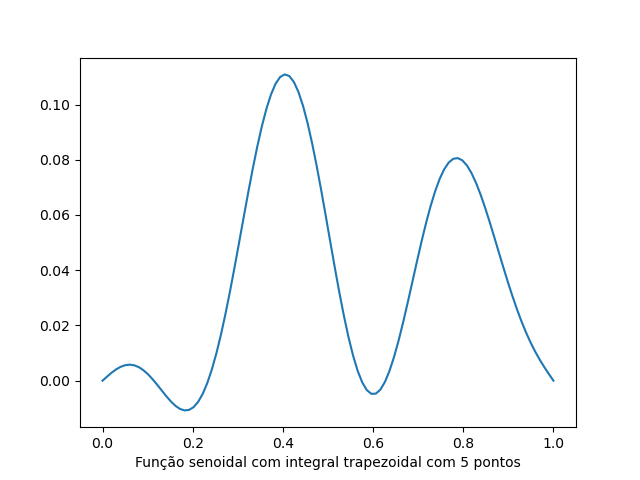
\includegraphics[width=1\textwidth]{exercicio6_seno.png}
\end{center}

\subsection{Parte (b)}
\begin{center}
    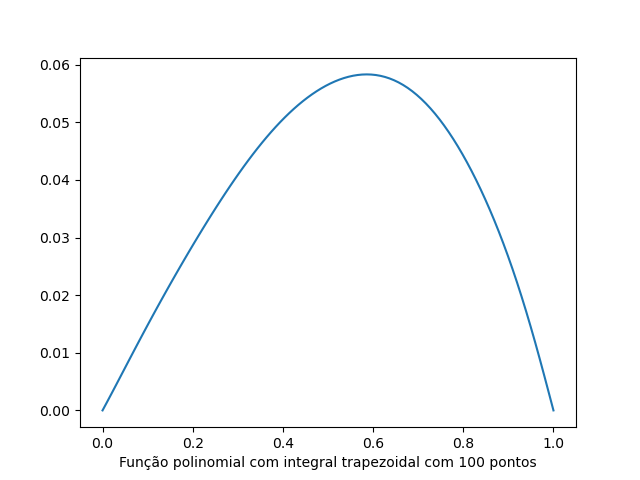
\includegraphics[width=1\textwidth]{exercicio6_polinomio.png}
\end{center}

Nesse caso, a função foi bem aproximada. Isso deve acontecer porque a aproximação da integral calculada com 100 pontos se aproxima muito melhor do valor analítico.

\section{Exercício 7}

\subsection{Parte (a)}
\[
J[v] = \frac{1}{2} \int_0^1 \left[ \alpha (v')^2 + \gamma v^2 \right] dx - \int_0^1 v dx.
\]

A condição de variação nula do funcional é obtida considerando uma perturbação \( v + \epsilon \eta \), onde \( \eta \in \mathcal{U} \) é uma função teste arbitrária e \( \epsilon \) é um parâmetro pequeno. A condição de variação nula é que a derivada de \( J[v + \epsilon \eta] \) com respeito a \( \epsilon \) seja zero em \( \epsilon = 0 \).

Primeiro, calculamos \( J[v + \epsilon \eta] \):
\[
J[v + \epsilon \eta] = \frac{1}{2} \int_0^1 \left[ \alpha ((v + \epsilon \eta)')^2 + \gamma (v + \epsilon \eta)^2 \right] dx - \int_0^1 (v + \epsilon \eta) dx.
\]

Expandindo e simplificando:
\[
J[v + \epsilon \eta] = \frac{1}{2} \int_0^1 \left[ \alpha (v' + \epsilon \eta')^2 + \gamma (v + \epsilon \eta)^2 \right] dx - \int_0^1 (v + \epsilon \eta) dx.
\]

\[
J[v + \epsilon \eta] = \frac{1}{2} \int_0^1 \left[ \alpha (v'^2 + 2 \epsilon v' \eta' + \epsilon^2 \eta'^2) + \gamma (v^2 + 2 \epsilon v \eta + \epsilon^2 \eta^2) \right] dx - \int_0^1 (v + \epsilon \eta) dx.
\]

A condição de variação nula é obtida ao tomar a derivada com respeito a \( \epsilon \) e avaliar em \( \epsilon = 0 \):
\[
\left. \frac{d}{d\epsilon} J[v + \epsilon \eta] \right|_{\epsilon=0} = 0.
\]

Calculamos a derivada:
\[
\left. \frac{d}{d\epsilon} J[v + \epsilon \eta] \right|_{\epsilon=0} = \int_0^1 \left[ \alpha v' \eta' + \gamma v \eta \right] dx - \int_0^1 \eta dx.
\]

Portanto, a formulação variacional é encontrar \( u \in \mathcal{U} \) tal que:
\[
\int_0^1 \left[ \alpha u' \eta' + \gamma u \eta \right] dx = \int_0^1 \eta dx \quad \forall \eta \in \mathcal{U}.
\]

\subsection{Parte (b)}

Primeiro, substituímos \( v = u + w \) no funcional \( J \):
\[
J[u + w] = \frac{1}{2} \int_0^1 \left[ \alpha ((u + w)')^2 + \gamma (u + w)^2 \right] dx - \int_0^1 (u + w) dx.
\]

Expandimos os termos dentro da integral:
\[
J[u + w] = \frac{1}{2} \int_0^1 \left[ \alpha (u' + w')^2 + \gamma (u + w)^2 \right] dx - \int_0^1 (u + w) dx.
\]

Separando os termos, obtemos:
\[
J[u + w] = \frac{1}{2} \int_0^1 \left[ \alpha (u'^2 + 2u'w' + w'^2) + \gamma (u^2 + 2uw + w^2) \right] dx - \int_0^1 (u + w) dx.
\]

Distribuindo a integral, obtemos:
\[
J[u + w] = \frac{1}{2} \int_0^1 \left[ \alpha u'^2 + 2\alpha u'w' + \alpha w'^2 + \gamma u^2 + 2\gamma uw + \gamma w^2 \right] dx - \int_0^1 u dx - \int_0^1 w dx.
\]

Reorganizando os termos, temos:
\[
J[u + w] = \frac{1}{2} \int_0^1 \left[ \alpha u'^2 + \gamma u^2 \right] dx + \frac{1}{2} \int_0^1 \left[ \alpha w'^2 + \gamma w^2 \right] dx + \int_0^1 \left[ \alpha u'w' + \gamma uw \right] dx - \int_0^1 u dx - \int_0^1 w dx.
\]

Utilizando a formulação variacional que encontramos anteriormente, sabemos que \( u \) minimiza \( J \), logo, a primeira variação é nula:
\[
\int_0^1 \left[ \alpha u' \eta' + \gamma u \eta \right] dx = \int_0^1 \eta dx \quad \forall \eta \in \mathcal{U}.
\]

Escolhendo \( \eta = w \), temos:
\[
\int_0^1 \left[ \alpha u' w' + \gamma u w \right] dx = \int_0^1 w dx.
\]

Portanto, a expressão para \( J[u + w] \) se simplifica para:
\[
J[u + w] = \frac{1}{2} \int_0^1 \left[ \alpha u'^2 + \gamma u^2 \right] dx + \frac{1}{2} \int_0^1 \left[ \alpha w'^2 + \gamma w^2 \right] dx + \int_0^1 w dx - \int_0^1 u dx - \int_0^1 w dx.
\]

Os termos \(\int_0^1 w dx\) se cancelam, restando:
\[
J[u + w] = J[u] + \frac{1}{2} \int_0^1 \left[ \alpha w'^2 + \gamma w^2 \right] dx.
\]

Como \(\alpha > 0\) e \(\gamma \geq 0\), o termo \(\frac{1}{2} \int_0^1 \left[ \alpha w'^2 + \gamma w^2 \right] dx \geq 0\).

Portanto:
\[
J[u + w] \geq J[u].
\]

\subsection{Parte (c)}
A equação de Euler-Lagrange para um funcional da forma:
\[
J[v] = \int_a^b L(x, v, v') \, dx
\]
é dada por:
\[
\frac{\partial L}{\partial v} - \frac{d}{dx} \left( \frac{\partial L}{\partial v'} \right) = 0.
\]

Para o nosso problema, o lagrangiano \( L \) é:
\[
L(x, v, v') = \frac{1}{2} \left[ \alpha (v')^2 + \gamma v^2 \right] - v.
\]

Calculamos as derivadas parciais:
\[
\frac{\partial L}{\partial v} = \gamma v - 1,
\]
\[
\frac{\partial L}{\partial v'} = \alpha v'.
\]

Calculamos a derivada total com respeito a \( x \):
\[
\frac{d}{dx} \left( \frac{\partial L}{\partial v'} \right) = \alpha v''.
\]

Substituímos na equação de Euler-Lagrange:
\[
\gamma v - 1 - \alpha v'' = 0,
\]
ou seja,
\[
\alpha v'' - \gamma v = -1.
\]

Portanto, a equação de Euler-Lagrange para o Problema M é:
\[
\alpha u'' - \gamma u = -1.
\]

Para resolver esta equação diferencial, consideramos a equação homogênea associada:
\[
\alpha u'' - \gamma u = 0.
\]

A solução geral da equação homogênea é:
\[
u_h(x) = C_1 e^{\sqrt{\frac{\gamma}{\alpha}} x} + C_2 e^{-\sqrt{\frac{\gamma}{\alpha}} x}.
\]

Para a equação completa, procuramos uma solução particular \( u_p \):
\[
\alpha u_p'' - \gamma u_p = -1.
\]

Tentamos uma solução particular constante \( u_p = A \):
\[
-\gamma A = -1 \quad \Rightarrow \quad A = \frac{1}{\gamma}.
\]

Portanto, a solução geral da equação diferencial é:
\[
u(x) = C_1 e^{\sqrt{\frac{\gamma}{\alpha}} x} + C_2 e^{-\sqrt{\frac{\gamma}{\alpha}} x} + \frac{1}{\gamma}.
\]

Aplicamos as condições de contorno \( u(0) = 1 \) e \( u(1) = 0 \):

1. Para \( u(0) = 1 \):
\[
C_1 + C_2 + \frac{1}{\gamma} = 1.
\]

2. Para \( u(1) = 0 \):
\[
C_1 e^{\sqrt{\frac{\gamma}{\alpha}}} + C_2 e^{-\sqrt{\frac{\gamma}{\alpha}}} + \frac{1}{\gamma} = 0.
\]

Resolvendo este sistema de equações lineares para \( C_1 \) e \( C_2 \):

\[
\begin{cases}
C_1 + C_2 = 1 - \frac{1}{\gamma}, \\
C_1 e^{\sqrt{\frac{\gamma}{\alpha}}} + C_2 e^{-\sqrt{\frac{\gamma}{\alpha}}} = -\frac{1}{\gamma}.
\end{cases}
\]

E assim determinamos as contantes:

\[
C_1 = \frac{e^{-\sqrt{\frac{\gamma}{\alpha}}} \left( -\frac{1}{\gamma} \right) - (1 - \frac{1}{\gamma}) e^{-\sqrt{\frac{\gamma}{\alpha}}}}{e^{\sqrt{\frac{\gamma}{\alpha}}} - e^{-\sqrt{\frac{\gamma}{\alpha}}}},
\]
\[
C_2 = \frac{e^{\sqrt{\frac{\gamma}{\alpha}}} \left( -\frac{1}{\gamma} \right) - (1 - \frac{1}{\gamma}) e^{\sqrt{\frac{\gamma}{\alpha}}}}{e^{-\sqrt{\frac{\gamma}{\alpha}}} - e^{\sqrt{\frac{\gamma}{\alpha}}}}.
\]

\section{Exercício 8}

Para resolver a equação de Euler-Lagrange para os casos dados:

1. \( \alpha = 1 \), \( \gamma = 1 \)
2. \( \alpha = 1 \times 10^{-5} \), \( \gamma = 1 \)

A equação de Euler-Lagrange é:
\[ \alpha u'' - \gamma u = -1 \]

Caso (a): \(\alpha = 1\), \(\gamma = 1\)

\[ u(x) = \frac{-e^{1 - x} - e^x + 1 + e}{1 + e} \]

\begin{center}
    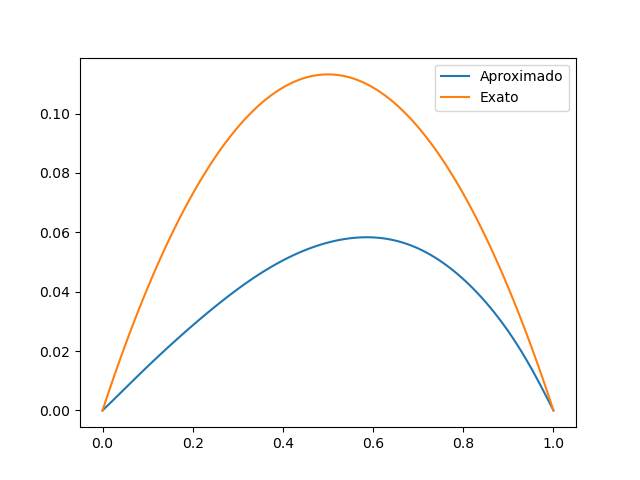
\includegraphics[width=1\textwidth]{exercicio8_alpha_grande.png}
\end{center}


Caso (b): \(\alpha = 1 \times 10^{-5}\), \(\gamma = 1\)

\[ u(x) = \frac{-e^{-100 \sqrt{10} (x - 1)} - e^{100 \sqrt{10} x} + 1 + e^{100 \sqrt{10}}}{1 + e^{100 \sqrt{10}}} \]

\begin{center}
    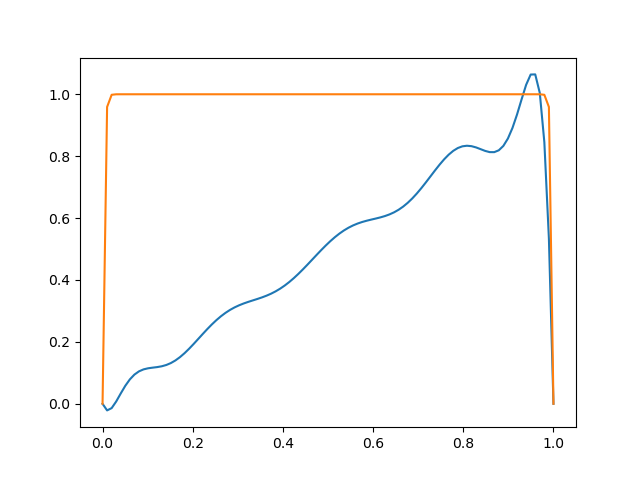
\includegraphics[width=1\textwidth]{exercicio8_alpha_pequeno.png}
\end{center}

\section{Exercício 9}
\subsection{Parte (a)}

Primeiro, calculamos \( J[u + \epsilon \eta] \):
\[
J[u + \epsilon \eta] = \frac{1}{2} \int_\Omega \left[ \alpha |\nabla (u + \epsilon \eta)|^2 + \gamma (u + \epsilon \eta)^2 \right] d\Omega - \int_\Omega f (u + \epsilon \eta) d\Omega - \int_{\Gamma_N} g (u + \epsilon \eta) d\Gamma.
\]

Expandindo e simplificando:
\[
J[u + \epsilon \eta] = \frac{1}{2} \int_\Omega \left[ \alpha (|\nabla u|^2 + 2 \epsilon \nabla u \cdot \nabla \eta + \epsilon^2 |\nabla \eta|^2) + \gamma (u^2 + 2 \epsilon u \eta + \epsilon^2 \eta^2) \right] d\Omega - \int_\Omega f (u + \epsilon \eta) d\Omega - \int_{\Gamma_N} g (u + \epsilon \eta) d\Gamma.
\]

A condição de variação nula é obtida ao tomar a derivada com respeito a \( \epsilon \) e avaliar em \( \epsilon = 0 \):
\[
\left. \frac{d}{d\epsilon} J[u + \epsilon \eta] \right|_{\epsilon=0} = 0.
\]

Calculamos a derivada:
\[
\left. \frac{d}{d\epsilon} J[u + \epsilon \eta] \right|_{\epsilon=0} = \int_\Omega \left[ \alpha \nabla u \cdot \nabla \eta + \gamma u \eta \right] d\Omega - \int_\Omega f \eta d\Omega - \int_{\Gamma_N} g \eta d\Gamma.
\]

Portanto, a formulação variacional é encontrar \( u \in \mathcal{U} \) tal que:
\[
\int_\Omega \left[ \alpha \nabla u \cdot \nabla \eta + \gamma u \eta \right] d\Omega = \int_\Omega f \eta d\Omega + \int_{\Gamma_N} g \eta d\Gamma \quad \forall \eta \in \mathcal{U}.
\]

\subsection{Parte (b)}

Para o nosso problema, o lagrangiano \( L \) é:
\[
L(u, \nabla u) = \frac{1}{2} \left[ \alpha |\nabla u|^2 + \gamma u^2 \right] - f u - g u \quad \text{em} \quad \Gamma_N.
\]

Calculamos as derivadas parciais:
\[
\frac{\partial L}{\partial u} = \gamma u - f,
\]
\[
\frac{\partial L}{\partial \nabla u} = \alpha \nabla u.
\]

Calculamos a divergência:
\[
\nabla \cdot \left( \frac{\partial L}{\partial \nabla u} \right) = \nabla \cdot (\alpha \nabla u) = \alpha \Delta u \quad \text{(onde} \quad \Delta = \nabla \cdot \nabla \text{ é o operador Laplaciano)}.
\]

Substituímos na equação de Euler-Lagrange:
\[
\gamma u - f - \alpha \Delta u = 0.
\]

Portanto, a equação de Euler-Lagrange é:
\[
\alpha \Delta u - \gamma u + f = 0.
\]

Forma Forte

Para encontrar a forma forte equivalente, incluindo as condições de contorno, reescrevemos a equação diferencial juntamente com as condições de contorno. Consideramos a equação:
\[
\alpha \Delta u - \gamma u + f = 0 \quad \text{em} \quad \Omega.
\]

Condições de Contorno

1. **Condição de Dirichlet**: \( u = 0 \) em \( \Gamma_D \).
2. **Condição de Neumann**: \(\frac{\partial u}{\partial n} = g\) em \( \Gamma_N \), onde \( \frac{\partial u}{\partial n} \) representa a derivada normal de \( u \) na fronteira \( \Gamma_N \).

Equação Completa

Portanto, a forma forte do problema é:
\[
\begin{cases}
\alpha \Delta u - \gamma u + f = 0 & \text{em} \quad \Omega, \\
u = 0 & \text{em} \quad \Gamma_D, \\
\alpha \frac{\partial u}{\partial n} = g & \text{em} \quad \Gamma_N.
\end{cases}
\]

\section{Exercício 10}

\begin{center}
    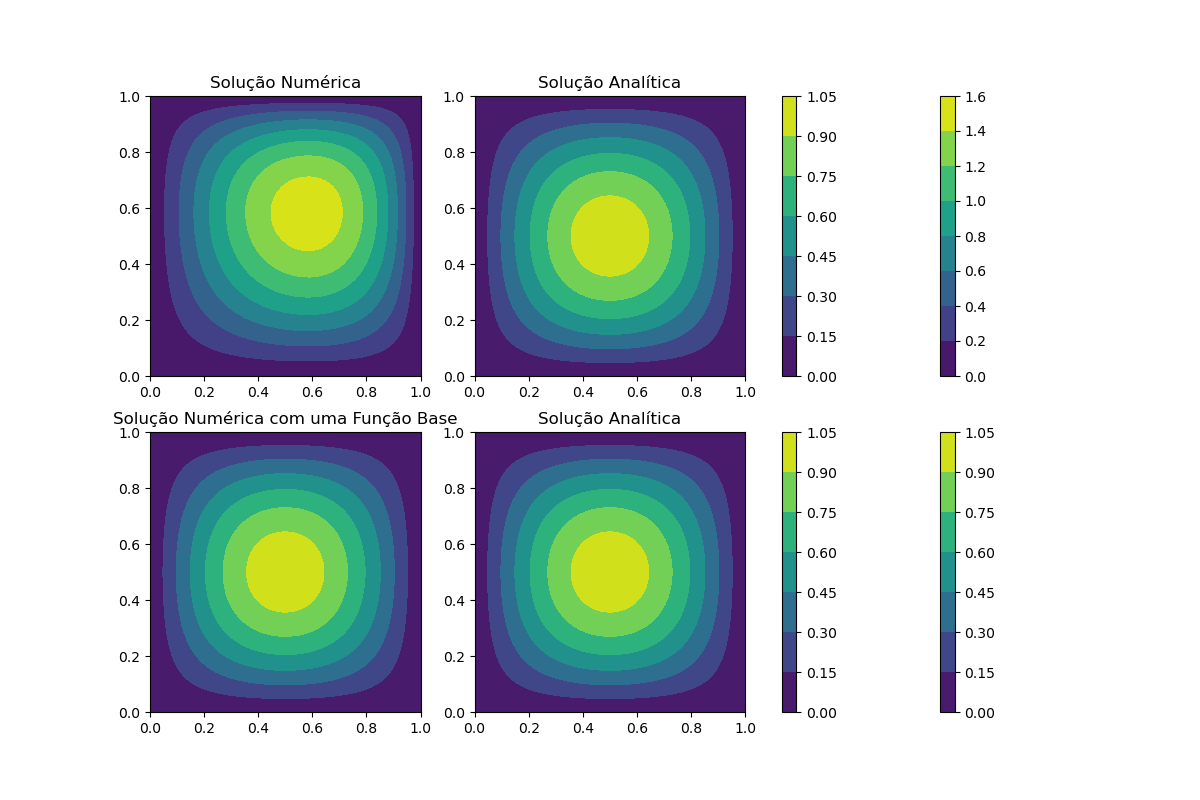
\includegraphics[width=1\textwidth]{exercicio10.png}
\end{center}

Podemos observar que a base de uma função se aproximou melhor da solução analítica. Isso se deve ao fato de que essa função tem o formato da solução analítica, enquanto que as bases polinomiais não tem.

\section{Exercício 11}

\subsection{Parte (b)}

Para um elemento linear com dois nós, utilizamos as funções de forma padrão:
\[
\phi_1(x) = 1 - x, \quad \phi_2(x) = x, \quad \text{para} \quad x \in [0, 1].
\]

A matriz de rigidez \( K \) é dada por:
\[
K_{ij} = \int_0^1 (\alpha \phi_i' \phi_j' + \gamma \phi_i \phi_j) \, dx.
\]

Calculamos os elementos de \( K \):

1. \( K_{11} \):
\[
K_{11} = \int_0^1 (\alpha \phi_1' \phi_1' + \gamma \phi_1 \phi_1) \, dx = \int_0^1 (\alpha (-1)(-1) + \gamma (1-x)^2) \, dx = \alpha \int_0^1 1 \, dx + \gamma \int_0^1 (1 - 2x + x^2) \, dx.
\]
\[
K_{11} = \alpha \left[ x \right]_0^1 + \gamma \left[ x - x^2 + \frac{x^3}{3} \right]_0^1 = \alpha (1 - 0) + \gamma \left(1 - 1 + \frac{1}{3}\right) = \alpha + \frac{\gamma}{3}.
\]

2. \( K_{12} \) e \( K_{21} \):
\[
K_{12} = \int_0^1 (\alpha \phi_1' \phi_2' + \gamma \phi_1 \phi_2) \, dx = \int_0^1 (\alpha (-1)(1) + \gamma (1-x)x) \, dx = -\alpha \int_0^1 1 \, dx + \gamma \int_0^1 (x - x^2) \, dx.
\]
\[
K_{12} = -\alpha \left[ x \right]_0^1 + \gamma \left[ \frac{x^2}{2} - \frac{x^3}{3} \right]_0^1 = -\alpha (1 - 0) + \gamma \left(\frac{1}{2} - \frac{1}{3}\right) = -\alpha + \frac{\gamma}{6}.
\]
\[
K_{21} = K_{12}.
\]

3. \( K_{22} \):
\[
K_{22} = \int_0^1 (\alpha \phi_2' \phi_2' + \gamma \phi_2 \phi_2) \, dx = \int_0^1 (\alpha (1)(1) + \gamma x^2) \, dx = \alpha \int_0^1 1 \, dx + \gamma \int_0^1 x^2 \, dx.
\]
\[
K_{22} = \alpha \left[ x \right]_0^1 + \gamma \left[ \frac{x^3}{3} \right]_0^1 = \alpha (1 - 0) + \gamma \frac{1}{3} = \alpha + \frac{\gamma}{3}.
\]

Portanto, a matriz de rigidez \( K \) é:
\[
K = \begin{bmatrix}
\alpha + \frac{\gamma}{3} & -\alpha + \frac{\gamma}{6} \\
-\alpha + \frac{\gamma}{6} & \alpha + \frac{\gamma}{3}
\end{bmatrix}.
\]

O vetor de carga \( F \) é dado por:
\[
F_i = \int_0^1 \phi_i \, dx.
\]

Calculamos os elementos de \( F \):

1. \( F_1 \):
\[
F_1 = \int_0^1 (1 - x) \, dx = \left[ x - \frac{x^2}{2} \right]_0^1 = 1 - \frac{1}{2} = \frac{1}{2}.
\]

2. \( F_2 \):
\[
F_2 = \int_0^1 x \, dx = \left[ \frac{x^2}{2} \right]_0^1 = \frac{1}{2}.
\]

Portanto, o vetor de carga \( F \) é:
\[
F = \begin{bmatrix}
\frac{1}{2} \\
\frac{1}{2}
\end{bmatrix}.
\]

\subsection{Parte (b)}

Para um elemento quadrático com três nós, utilizamos as funções de forma padrão:
\[
\phi_1(x) = 2(x - 0.5)(x - 1), \quad \phi_2(x) = -4x(x - 1), \quad \phi_3(x) = 2x(x - 0.5), \quad \text{para} \quad x \in [0, 1].
\]

A matriz de rigidez \( K \) é dada por:
\[
K_{ij} = \int_0^1 (\alpha \phi_i' \phi_j' + \gamma \phi_i \phi_j) \, dx.
\]

Para simplificar, podemos calcular os elementos de \( K \) e \( F \) utilizando uma abordagem numérica (por exemplo, quadratura de Gauss). Aqui eu utilizei uma biblioteca de matemática simbólica, o sympy, para calcular essa matriz, e obtive:

\[
K = \begin{bmatrix}
    2.3*alpha + 0.13*gamma & -2.7*alpha + 0.067*gamma & 0.33*alpha - 0.033*gamma \\
    -2.7*alpha + 0.067*gamma & 5.3*alpha + 0.53*gamma & -2.7*alpha + 0.067*gamma \\
    0.33*alpha - 0.033*gamma & -2.7*alpha + 0.067*gamma & 2.3*alpha + 0.13*gamma
\end{bmatrix}
\]

\[
F = \begin{bmatrix}
    0.17 \\
    0.67 \\
    0.17
\end{bmatrix}
\]

\section{Exercício 12}

Para uma partição uniforme do domínio \(\Omega = (0, 1)\) em \(n\) elementos finitos lineares, temos \(x_i = \frac{i}{n}\), para \(i = 0, 1, \ldots, n\).

 Funções de forma lineares

Para cada elemento \(\Omega_i = (x_i, x_{i+1})\), as funções de forma lineares são:
\[
\phi_i(x) = \frac{x_{i+1} - x}{x_{i+1} - x_i}, \quad \phi_{i+1}(x) = \frac{x - x_i}{x_{i+1} - x_i}.
\]

 Matriz de rigidez local

Para calcular a matriz de rigidez local \(K^e\) em cada elemento \(\Omega_i\), utilizamos:
\[
K^e_{ij} = \int_{x_i}^{x_{i+1}} (\alpha \phi_i' \phi_j' + \gamma \phi_i \phi_j) \, dx.
\]

As derivadas das funções de forma são constantes em cada elemento:
\[
\phi_i' = -\frac{1}{h}, \quad \phi_{i+1}' = \frac{1}{h}, \quad \text{onde} \quad h = \frac{1}{n}.
\]

Portanto, temos:
\[
K^e = \begin{bmatrix}
\int_{x_i}^{x_{i+1}} \left( \alpha \left( -\frac{1}{h} \right) \left( -\frac{1}{h} \right) + \gamma \left( \frac{x_{i+1} - x}{h} \right) \left( \frac{x_{i+1} - x}{h} \right) \right) dx & \int_{x_i}^{x_{i+1}} \left( \alpha \left( -\frac{1}{h} \right) \left( \frac{1}{h} \right) + \gamma \left( \frac{x_{i+1} - x}{h} \right) \left( \frac{x - x_i}{h} \right) \right) dx \\
\int_{x_i}^{x_{i+1}} \left( \alpha \left( \frac{1}{h} \right) \left( -\frac{1}{h} \right) + \gamma \left( \frac{x - x_i}{h} \right) \left( \frac{x_{i+1} - x}{h} \right) \right) dx & \int_{x_i}^{x_{i+1}} \left( \alpha \left( \frac{1}{h} \right) \left( \frac{1}{h} \right) + \gamma \left( \frac{x - x_i}{h} \right) \left( \frac{x - x_i}{h} \right) \right) dx
\end{bmatrix}.
\]

Após simplificação, obtemos:
\[
K^e = \begin{bmatrix}
\frac{\alpha}{h} + \frac{\gamma h}{3} & -\frac{\alpha}{h} + \frac{\gamma h}{6} \\
-\frac{\alpha}{h} + \frac{\gamma h}{6} & \frac{\alpha}{h} + \frac{\gamma h}{3}
\end{bmatrix}.
\]

 Vetor de carga local

Para o vetor de carga local \(F^e\), temos:
\[
F^e_i = \int_{x_i}^{x_{i+1}} \phi_i \, dx.
\]

Calculamos os elementos de \(F^e\):
\[
F^e = \begin{bmatrix}
\int_{x_i}^{x_{i+1}} \frac{x_{i+1} - x}{h} \, dx \\
\int_{x_i}^{x_{i+1}} \frac{x - x_i}{h} \, dx
\end{bmatrix}.
\]

Após simplificação, obtemos:
\[
F^e = \begin{bmatrix}
\frac{h}{2} \\
\frac{h}{2}
\end{bmatrix}.
\]

 Montagem da matriz global

A matriz de rigidez global \(K\) é montada somando as contribuições dos elementos locais \(K^e\) nos graus de liberdade correspondentes:
\[
K = \begin{bmatrix}
\frac{\alpha}{h} + \frac{\gamma h}{3} & -\frac{\alpha}{h} + \frac{\gamma h}{6} & 0 & \cdots & 0 \\
-\frac{\alpha}{h} + \frac{\gamma h}{6} & 2\left(\frac{\alpha}{h} + \frac{\gamma h}{3}\right) & -\frac{\alpha}{h} + \frac{\gamma h}{6} & \cdots & 0 \\
0 & -\frac{\alpha}{h} + \frac{\gamma h}{6} & 2\left(\frac{\alpha}{h} + \frac{\gamma h}{3}\right) & \cdots & 0 \\
\vdots & \vdots & \vdots & \ddots & -\frac{\alpha}{h} + \frac{\gamma h}{6} \\
0 & 0 & 0 & -\frac{\alpha}{h} + \frac{\gamma h}{6} & \frac{\alpha}{h} + \frac{\gamma h}{3}
\end{bmatrix}.
\]

 Vetor de carga global

O vetor de carga global \(F\) é montado somando as contribuições dos elementos locais \(F^e\):
\[
F = \begin{bmatrix}
\frac{h}{2} \\
h \\
h \\
\vdots \\
h \\
\frac{h}{2}
\end{bmatrix}.
\]

 Conclusão

A matriz de rigidez resultante é tridiagonal, com os seguintes coeficientes:
\[
K_{ii} = 2\left(\frac{\alpha}{h} + \frac{\gamma h}{3}\right) \quad \text{para} \quad i = 1, \ldots, n-1,
\]
\[
K_{i,i+1} = K_{i+1,i} = -\frac{\alpha}{h} + \frac{\gamma h}{6} \quad \text{para} \quad i = 1, \ldots, n-1.
\]

O vetor de carga tem os seguintes coeficientes:
\[
F_1 = F_n = \frac{h}{2}, \quad F_i = h \quad \text{para} \quad i = 2, \ldots, n-1.
\]

\section{Exercício 13}

Para encontrar a equação de Euler-Lagrange do Problema V, consideramos a formulação variacional:
\[
\int_0^1 (\alpha u'v' + u v) \, dx = \int_0^1 v \, dx \quad \forall v \in \mathcal{U},
\]
onde \(\mathcal{U} = H^1_0(0,1)\).

A equação de Euler-Lagrange associada a este problema é obtida aplicando o método das variações. O funcional associado é:
\[
J[u] = \frac{1}{2} \int_0^1 (\alpha u'^2 + u^2) \, dx - \int_0^1 u \, dx.
\]

A equação de Euler-Lagrange para um funcional da forma:
\[
J[u] = \int_a^b L(x, u, u') \, dx
\]
é dada por:
\[
\frac{\partial L}{\partial u} - \frac{d}{dx} \left( \frac{\partial L}{\partial u'} \right) = 0.
\]

Para o nosso problema, o Lagrangiano \( L \) é:
\[
L(u, u') = \frac{1}{2} (\alpha u'^2 + u^2) - u.
\]

Calculamos as derivadas parciais:
\[
\frac{\partial L}{\partial u} = u - 1,
\]
\[
\frac{\partial L}{\partial u'} = \alpha u'.
\]

Calculamos a derivada total com respeito a \(x\):
\[
\frac{d}{dx} \left( \frac{\partial L}{\partial u'} \right) = \alpha u''.
\]

Substituímos na equação de Euler-Lagrange:
\[
u - 1 - \alpha u'' = 0,
\]
ou seja,
\[
\alpha u'' - u = -1.
\]

Portanto, a equação de Euler-Lagrange é:
\[
\alpha u'' - u = -1.
\]

Que tem como solução:

\[
u(x) = -\frac{1}{e^{\sqrt{\frac{1}{\alpha}}} - e^{-\sqrt{\frac{1}{\alpha}}}} e^{\sqrt{\frac{1}{\alpha}} x} + \left(-1 + \frac{1}{e^{\sqrt{\frac{1}{\alpha}}} - e^{-\sqrt{\frac{1}{\alpha}}}}\right) e^{-\sqrt{\frac{1}{\alpha}} x} + 1.
\]


\end{document}